% !TEX root = demo.tex
\section{Demonstration}
In this section, we detail the proposed demonstration.
The objective of this demonstration is to illustrate 
how \sys enables the rapid iterative construction of data cleaning plans
and the ability to transfer workflows between similar dirty datasets.

\subsection{Datasets}
In the demo, we will consider cleaning workflows on three different datasets.
The first dataset contains 858 Zagat reviews\footnote{\scriptsize{ \url{cs.utexas.edu/users/ml/riddle/data/restaurant.tar.gz}}},
each tagged with the cuisine of the restaurant reviewed (e.g. ``Chinese" or ``French").
The second dataset, which is similar to the first, is from Yelp \footnote{\scriptsize{\url{https://www.yelp.com/academic_dataset}}} and contains 58,127 restaurant records that are also tagged with a category.
The third dataset consists of $3,049,914$ records of liquor sales from the state of Iowa\footnote{\scriptsize{\url{data.iowa.gov/Economy/Iowa-Liquor-Sales/m3tr-qhgy}}}, including the store where the purchase occurred and the items and cost of the purchase.
In all three datasets, categorical columns are inconsistent across records (e.g. cuisine tags for ``Chinese" vs. ``Chinese Cuisine"), records are duplicated, and formatting errors abound. 
We will use \sys to resolve these errors using Extraction and Entity Resolution, then run aggregate queries over the cleaned datasets.

\begin{figure}[t]
\centering
 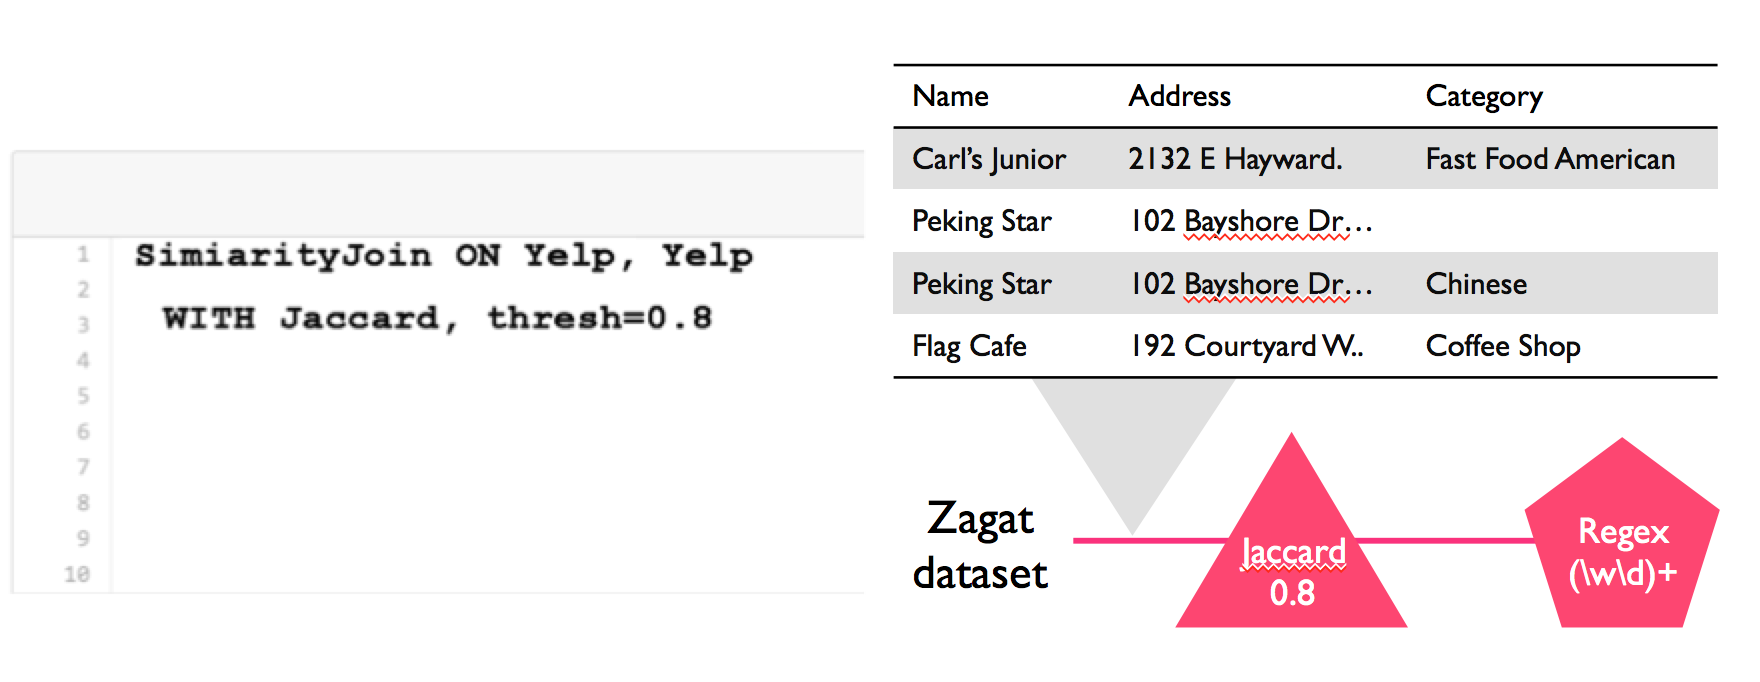
\includegraphics[width=\columnwidth]{figs/dashboard_screenshot.png}
 \caption{The dashboard contains both a visual interface and a text box to specify data cleaning operations. When the user is satisfied, she can run the plan and see the results on the right. \label{screenshot}}
\end{figure}


\begin{figure}[t]
\centering
 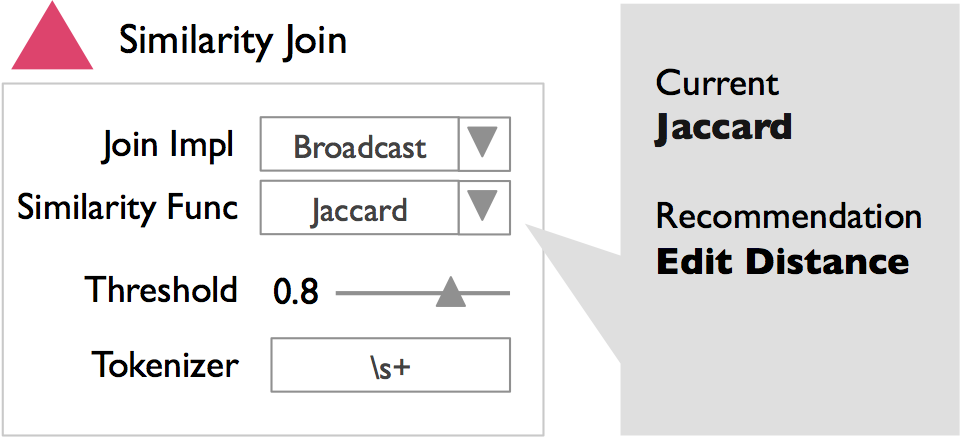
\includegraphics[width=0.8\columnwidth]{figs/dashboard_recsys.png}
 \caption{The operator view lists the parameters of an operator. Users can view recommended changes and modify parameters on the fly.}
 \label{screenshot-rec}
 \vspace{-0.4cm}
\end{figure}

\subsection{Demo Walkthrough}
Below, we detail the steps of the proposed demonstration.
A screenshot of the dashboard interface is illustrated in Figure~\ref{screenshot}.

\vspace{0.2em}

\noindent\textbf{Step 1: } Participants will select a dataset (e.g., the Zagat dataset), and load a pre-populated data cleaning plan and target query for it.
Participants must first extract the columns of the dataset into the proper schema using a regex-based Extraction.
Then, participants will be able to manually tune the Enity Resolution by choosing between Similarity Join implementations, adjusting the thresholds for the Similarity Join, and adding a crowdsourced filtering step.

\vspace{0.2em}

\noindent\textbf{Step 2: } At all times, the interface will display a representative sample of the cleaning plan's input and output and the results of the target query so that the participant can see how cleaning affects the data. 
If a plan modification adds crowdsourcing, participants can complete crowd tasks in \sys's crowd interface.

\vspace{0.2em}

\noindent\textbf{Step 3:} Participants re-evaluate and adjust their plan by clicking on an operator (Figure~\ref{screenshot-rec}).
This view will show the system's recommended changes to the operator and allow the participant to make those changes easily.
For example, Figure~\ref{screenshot-rec} shows a recommendation to change the similarity metric from Jaccard to Edit Distance since the attribute in question does not have many tokens.

\vspace{0.2em}

\noindent\textbf{Step 4: } Participants can then switch datasets. Switching between restaurant datasets (Zagat and Yelp) demonstrates reuse of the same plan on novel data, while switching to the alcohol dataset demonstrates that \sys is effective across data domains.
